\documentclass[10pt]{article}
\usepackage[margin=0.7in]{geometry}
\usepackage{times}
\usepackage{amsmath,amssymb}
\usepackage{booktabs,tabularx,array}
\usepackage{enumitem}
\usepackage{microtype}
\usepackage{hyperref}
\usepackage{tikz}
\usetikzlibrary{arrows.meta,positioning,fit,calc,shapes.geometric}
\hypersetup{hidelinks}
\newcolumntype{Y}{>{\raggedright\arraybackslash}X}
\setlist{nosep,leftmargin=1.4em}

\definecolor{loopcol}{RGB}{216,140,30}
\definecolor{chunkcol}{RGB}{183,83,42}
\definecolor{landmarkcol}{RGB}{42,104,155}
\definecolor{gridcol}{RGB}{120,120,120}
\definecolor{pathcol}{RGB}{190,55,55}

\tikzset{
  st/.style={circle,draw,minimum size=7mm,inner sep=0pt,font=\small\bfseries},
  corner/.style={st,fill=loopcol!18,draw=loopcol,line width=1pt},
  ge/.style={-,draw=gridcol!55,line width=0.7pt},
  le/.style={-{Stealth[length=4pt]},draw=loopcol,line width=1.3pt},
  ce/.style={-{Stealth[length=4pt]},draw=chunkcol,line width=1.3pt},
  de/.style={-{Stealth[length=4pt]},draw=landmarkcol,line width=1.3pt}
}

\title{Two Normative Agents That Walk the Same Paths:\\
A Chunk--Landmark Twin Pair on the Full Search Task Set\\
\large Analysis 10: per-trial trajectories over the 44 proposal-5 pairs,
and what they can and cannot identify}
\author{}
\date{6 June 2026}

\begin{document}
\maketitle

\begin{abstract}
We pair a normative action-chunk agent with a normative landmark/state agent on the
canonical proposal-5 search task---a $3\times3$ grid with a one-way clockwise corner loop
$1\to3\to9\to7\to1$---and compute the trajectory each chooses on \emph{every} one of the
44 ordered start--goal pairs in the locked task catalog. The chunk agent $T_1$ stores a
single grammar element, the loop bigram $\textsc{loop}^2$; the landmark agent $S_2$ stores
four memorized corner-to-corner shortcuts $1\!\to\!9,3\!\to\!7,9\!\to\!1,7\!\to\!3$. The
central result is computational: $T_1$ and $S_2$ select \textbf{identical primitive
trajectories on all 44 pairs}, under both cost conventions of analysis-5. Trajectories
therefore cannot separate action-chunk from landmark abstraction. The 12 loop-dominant
trials separate loop-knowers from loop-naive planners; the 8 tie trials separate
loop-biased from grid-biased route preference; neither separates the chunk--landmark twin.
We give the minimal recoverable trial set---a small battery of loop-dominant trials, tie
trials, a corner-generalization manipulation, and successor/chunk judgments---that does
break the aliasing. (The graph here is the locked task graph; the schematic mid-edge loop
used in Analysis~9 is superseded for task-set work.)
\end{abstract}

\section{The canonical task and its trial catalog}

The latent task is the retained $3\times3$ + directed-loop topology
(Fig.~\ref{fig:task}). Grid actions $\{\textsf{L},\textsf{R},\textsf{U},\textsf{D}\}$ move
between four-neighbours in both directions; the loop action $\textsc{loop}$ is a one-way
clockwise cycle on the corners, $1\to3\to9\to7\to1$, available only at corners
$\{1,3,7,9\}$. Two consecutive loops reach the diagonally opposite corner in two steps,
where any grid route needs four:
\[
\textsc{loop}^2:\quad 1\to9,\quad 3\to7,\quad 9\to1,\quad 7\to3 .
\]

\begin{figure}[htbp]
\centering
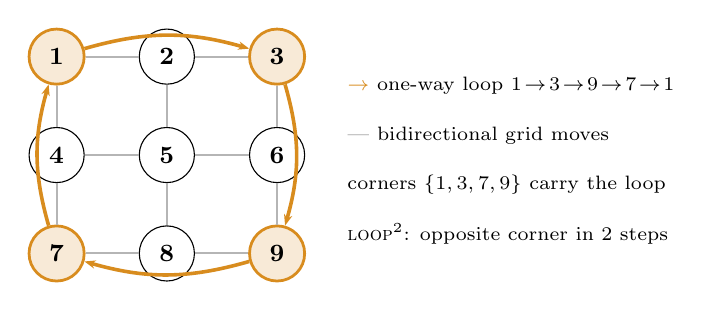
\begin{tikzpicture}[x=1.4cm,y=1.25cm]
  \node[corner] (1) at (0,2){1}; \node[st](2) at (1,2){2}; \node[corner](3) at (2,2){3};
  \node[st](4) at (0,1){4};       \node[st](5) at (1,1){5}; \node[st](6) at (2,1){6};
  \node[corner](7) at (0,0){7};   \node[st](8) at (1,0){8}; \node[corner](9) at (2,0){9};
  \foreach \a/\b in {1/2,2/3,4/5,5/6,7/8,8/9,1/4,4/7,2/5,5/8,3/6,6/9}{\draw[ge](\a)--(\b);}
  \draw[le] (1) to[bend left=16] (3);
  \draw[le] (3) to[bend left=16] (9);
  \draw[le] (9) to[bend left=16] (7);
  \draw[le] (7) to[bend left=16] (1);
  \node[anchor=west,font=\scriptsize] at (2.55,1.7){\textcolor{loopcol}{$\rightarrow$} one-way loop $1\!\to\!3\!\to\!9\!\to\!7\!\to\!1$};
  \node[anchor=west,font=\scriptsize] at (2.55,1.2){\textcolor{gridcol}{---} bidirectional grid moves};
  \node[anchor=west,font=\scriptsize] at (2.55,0.7){corners $\{1,3,7,9\}$ carry the loop};
  \node[anchor=west,font=\scriptsize] at (2.55,0.2){$\textsc{loop}^2$: opposite corner in 2 steps};
\end{tikzpicture}
\caption{The proposal-5 task graph. Grid moves are bidirectional; the loop is a one-way
clockwise corner cycle. The diagnostic structure of the task lives entirely in the loop:
it is the only action that creates a learnable shortcut.}
\label{fig:task}
\end{figure}

The locked search catalog contains 44 nontrivial ordered pairs, stratified by comparing
the grid-only distance $d_{\mathrm{grid}}$ with the loop-using distance $d_{\mathrm{loop}}$:
\begin{center}\small
\begin{tabular}{@{}lcl@{}}
\toprule
Stratum & Count & Definition \\
\midrule
grid-dominant & 24 & $d_{\mathrm{grid}}<d_{\mathrm{loop}}$ (the loop is a detour) \\
loop-dominant & 12 & $d_{\mathrm{loop}}<d_{\mathrm{grid}}$ (the loop is a shortcut) \\
tie           & 8  & $d_{\mathrm{grid}}=d_{\mathrm{loop}}$ (equal length; route is a choice) \\
\bottomrule
\end{tabular}
\end{center}
Each session draws 7 grid-dominant, 7 loop-dominant, and 10 tie trials.

\section{The two normative families and the closest twin}

The project fixes two normative agent families on this graph (\texttt{agent-definitions},
analysis-5). Each agent stores a discrete structure; the optimal goal-conditioned policy is
the solution of one shared semi-Markov Bellman recursion, read out by a softmax with
inverse temperature $\beta$.

\paragraph{Action-chunk (temporal) family.}
$T_0$ is the primitive planner with actions $\{\textsf{L},\textsf{R},\textsf{U},\textsf{D},
\textsc{loop}\}$. $T_1$ adds the single chunk $\textsc{loop}^2$; because a chunk is a
reusable grammar element, this \emph{one} element applies from all four corners, reaching
a different destination each time. $T_2$ adds the grid-diagonal bigrams
$\{\textsf{RD},\textsf{RU},\textsf{LD},\textsf{LU}\}$; $T_3$ adds both. Under the
analysis-5 utility ranking (Version~A, $\alpha\!\approx\!1$), $\textsc{loop}^2$ is the
uniquely useful chunk because it is the only bigram that reaches a state the primitives
cannot reach in the same number of steps.

\paragraph{Landmark/state family.}
$S_0$ knows only grid neighbours; $S_1$ adds the loop neighbours; $S_2$ adds the four
memorized diagonal corner shortcuts $1\!\to\!9,3\!\to\!7,9\!\to\!1,7\!\to\!3$ as
\emph{independent} stored routes. In the Analysis-7 vocabulary, $S_2$ is a landmark-option
agent: the landmarks are the corners $\mathcal L=\{1,3,7,9\}$, and the landmark edges are
the diagonal relations $\mathcal E^{\mathcal L}=\{(1,9),(3,7),(9,1),(7,3)\}$, each realized
through the primitive loop.

\paragraph{The closest twin.}
$T_1$ and $S_2$ induce the \emph{same} augmented transition graph: grid $+$ loop $+$ the
four diagonal corner edges. They therefore have the same optimal value function and the
same optimal paths. Their only difference is structural and is invisible to the path
itself: $T_1$ holds \emph{one} action-string element that generalizes across corners,
whereas $S_2$ holds \emph{four} independent state-to-state routes that happen to share an
action sequence (Fig.~\ref{fig:twin}). This is the action-chunk vs.\ landmark-option
contrast in its sharpest, most normatively reasonable form. A second, weaker twin pairs
$T_2$ (grid-diagonal bigrams) with an edge-based state agent storing the same grid
diagonals; we focus on $T_1$/$S_2$ because the loop makes it exact.

\begin{figure}[htbp]
\centering
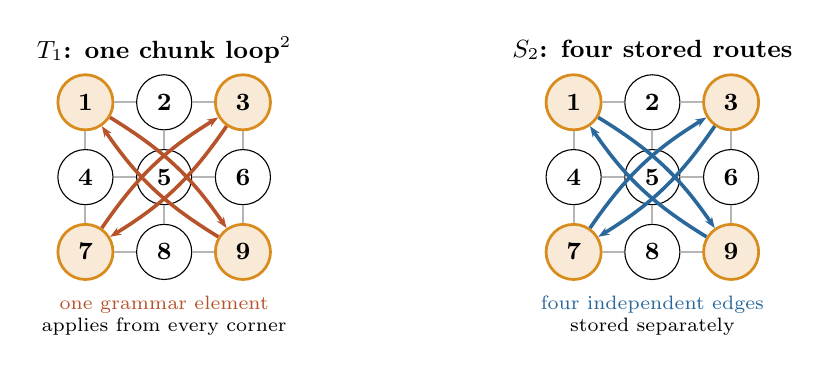
\begin{tikzpicture}[x=1.0cm,y=0.95cm]
\begin{scope}
  \node[font=\bfseries\small] at (1,2.7){$T_1$: one chunk $\textsc{loop}^2$};
  \node[corner](a1) at (0,2){1};\node[st](a2) at (1,2){2};\node[corner](a3) at (2,2){3};
  \node[st](a4) at (0,1){4};\node[st](a5) at (1,1){5};\node[st](a6) at (2,1){6};
  \node[corner](a7) at (0,0){7};\node[st](a8) at (1,0){8};\node[corner](a9) at (2,0){9};
  \foreach \a/\b in {a1/a2,a2/a3,a4/a5,a5/a6,a7/a8,a8/a9,a1/a4,a4/a7,a2/a5,a5/a8,a3/a6,a6/a9}{\draw[ge](\a)--(\b);}
  \draw[ce] (a1) to[bend left=12] (a9);
  \draw[ce] (a3) to[bend left=12] (a7);
  \draw[ce] (a9) to[bend left=12] (a1);
  \draw[ce] (a7) to[bend left=12] (a3);
  \node[font=\scriptsize,align=center] at (1,-0.85){\textcolor{chunkcol}{one grammar element}\\applies from every corner};
\end{scope}
\begin{scope}[xshift=6.2cm]
  \node[font=\bfseries\small] at (1,2.7){$S_2$: four stored routes};
  \node[corner](b1) at (0,2){1};\node[st](b2) at (1,2){2};\node[corner](b3) at (2,2){3};
  \node[st](b4) at (0,1){4};\node[st](b5) at (1,1){5};\node[st](b6) at (2,1){6};
  \node[corner](b7) at (0,0){7};\node[st](b8) at (1,0){8};\node[corner](b9) at (2,0){9};
  \foreach \a/\b in {b1/b2,b2/b3,b4/b5,b5/b6,b7/b8,b8/b9,b1/b4,b4/b7,b2/b5,b5/b8,b3/b6,b6/b9}{\draw[ge](\a)--(\b);}
  \draw[de] (b1) to[bend left=12] (b9);
  \draw[de] (b3) to[bend left=12] (b7);
  \draw[de] (b9) to[bend left=12] (b1);
  \draw[de] (b7) to[bend left=12] (b3);
  \node[font=\scriptsize,align=center] at (1,-0.85){\textcolor{landmarkcol}{four independent edges}\\stored separately};
\end{scope}
\end{tikzpicture}
\caption{The twin's only difference. Both agents add exactly the four diagonal corner
edges, so the induced map and every optimal path coincide. $T_1$ stores them as one
reusable action string; $S_2$ stores them as four separate state-to-state routes. The
difference is structural, not behavioural-on-path.}
\label{fig:twin}
\end{figure}

\section{Per-trial trajectories over the full task set}

We computed, for every agent and every pair, the optimal primitive trajectory (value
iteration on each agent's option graph; ties broken toward the agent's own abstraction).
The script and per-pair CSV are in \texttt{code/}. The headline is a single line.

\begin{quote}
\textbf{$T_1$ and $S_2$ choose the identical primitive trajectory on all 44/44 pairs}
(both cost conventions). On these trials the action-chunk and landmark agents are
behaviourally indistinguishable.
\end{quote}

What the trajectory \emph{does} reveal is loop usage, and only that. Every loop-knowing
agent ($T_0$--$T_3$, $S_1$, $S_2$) takes the short loop route on loop-dominant pairs; the
loop-naive $S_0$ takes a strictly longer grid detour. On grid-dominant pairs all agents
agree. On tie pairs, agents that favour the loop diagonal ($T_1,S_2,T_3$) take the loop
route while grid-favouring agents ($T_2,S_0$) take the grid route, at equal length.
Tables~\ref{tab:loop}--\ref{tab:tie} give the trajectories; the 24 grid-dominant pairs are
omitted because all agents take the same 2-step grid path there.

\begin{table}[htbp]
\centering\footnotesize
\begin{tabularx}{\textwidth}{@{}llccYY@{}}
\toprule
Pair & $s\!\to\!s_\star$ & $d_{\mathrm{grid}}$ & $d_{\mathrm{loop}}$ &
loop-knowers ($T_0$--$T_3$, $S_1$, $S_2$) & loop-naive $S_0$ \\
\midrule
L01 & $1\!\to\!6$ & 3 & 2 & 1-3-6 & 1-2-3-6 \\
L02 & $1\!\to\!9$ & 4 & 2 & 1-3-9 & 1-2-3-6-9 \\
L03 & $2\!\to\!9$ & 3 & 2 & 2-3-9 & 2-3-6-9 \\
L04 & $3\!\to\!7$ & 4 & 2 & 3-9-7 & 3-2-1-4-7 \\
L05 & $3\!\to\!8$ & 3 & 2 & 3-9-8 & 3-2-5-8 \\
L06 & $4\!\to\!3$ & 3 & 2 & 4-1-3 & 4-5-6-3 \\
L07 & $6\!\to\!7$ & 3 & 2 & 6-9-7 & 6-5-4-7 \\
L08 & $7\!\to\!2$ & 3 & 2 & 7-1-2 & 7-8-5-2 \\
L09 & $7\!\to\!3$ & 4 & 2 & 7-1-3 & 7-8-9-6-3 \\
L10 & $8\!\to\!1$ & 3 & 2 & 8-7-1 & 8-7-4-1 \\
L11 & $9\!\to\!1$ & 4 & 2 & 9-7-1 & 9-8-7-4-1 \\
L12 & $9\!\to\!4$ & 3 & 2 & 9-7-4 & 9-8-7-4 \\
\bottomrule
\end{tabularx}
\caption{The 12 loop-dominant trials. $T_1$ and $S_2$ (and all loop-knowers) take the
2-step loop route; the loop-naive $S_0$ is forced onto a 3--4 step grid detour. These
trials separate ``knows/uses the loop'' from ``does not''---not chunk from landmark.}
\label{tab:loop}
\end{table}

\begin{table}[htbp]
\centering\footnotesize
\begin{tabularx}{\textwidth}{@{}llYY@{}}
\toprule
Pair & $s\!\to\!s_\star$ & loop route ($T_1,S_2,T_3$ prefer) & grid route ($T_2,S_0$ prefer) \\
\midrule
T01 & $1\!\to\!8$ & 1-3-9-8 & 1-2-5-8 \\
T02 & $2\!\to\!7$ & 2-3-9-7 & 2-1-4-7 \\
T03 & $3\!\to\!4$ & 3-9-7-4 & 3-2-1-4 \\
T04 & $4\!\to\!9$ & 4-1-3-9 & 4-5-6-9 \\
T05 & $6\!\to\!1$ & 6-9-7-1 & 6-5-4-1 \\
T06 & $7\!\to\!6$ & 7-1-3-6 & 7-8-9-6 \\
T07 & $8\!\to\!3$ & 8-7-1-3 & 8-9-6-3 \\
T08 & $9\!\to\!2$ & 9-7-1-2 & 9-8-5-2 \\
\bottomrule
\end{tabularx}
\caption{The 8 tie trials ($d_{\mathrm{grid}}=d_{\mathrm{loop}}=3$). Both routes are
equally short, so the route taken is pure representational preference. $T_1$ and $S_2$ both
take the loop route; $T_2$ and $S_0$ take the grid route. The tie trials separate
loop-biased from grid-biased maps---but $T_1$ and $S_2$ still coincide.}
\label{tab:tie}
\end{table}

\section{What the trajectories can and cannot identify}

Reading the tables as a recovery instrument:
\begin{itemize}
\item \textbf{Grid-dominant trials (24): uninformative.} Every agent walks the same 2-step
grid path; nothing about representation is exposed.
\item \textbf{Loop-dominant trials (12): identify loop knowledge.} Taking the 2-step loop
versus a 3--4 step grid detour cleanly separates loop-knowers ($T_{1\text{--}3},S_1,S_2$)
from the loop-naive baseline $S_0$. This is a representation/competence contrast, not a
chunk-vs-landmark contrast.
\item \textbf{Tie trials (8): identify loop bias.} At equal length, choosing the loop
route versus the grid route separates loop-biased maps ($T_1,S_2,T_3$) from grid-biased
maps ($T_2$) and from an indifferent primitive planner ($T_0$, $50/50$).
\item \textbf{Nothing on path separates $T_1$ from $S_2$.} They are point-for-point
identical on all 44 pairs. The action-chunk and landmark-option hypotheses are
\emph{trajectory-aliased} on this task.
\end{itemize}
The aliasing is not a defect of the task; it is a precise statement of why behaviour alone
is insufficient and why the project needs structure-level inference and auxiliary probes.

\section{Cognitive maps of the twin}

Both agents warp the cognitive map into the same ``diamond'': the four corners are pulled
together because each diagonal pair is one cognitive step apart
(Fig.~\ref{fig:twin}). The representational-dissimilarity geometry is therefore nearly
identical for $T_1$ and $S_2$, which is the map-level counterpart of the trajectory
aliasing. The difference is in \emph{where the contraction comes from}: for $T_1$ it is a
single action-string relation that should contract \emph{all four} corner pairs uniformly
and should transfer to any corner where $\textsc{loop}^2$ is executable; for $S_2$ it is
four independently stored edges that contract only the specifically learned pairs. This is
the wedge the recovery design must drive into.

\section{Minimal recoverable trial set}

Trajectory aliasing means the recoverable design is layered. Each layer targets a contrast
the previous one cannot resolve.

\begin{description}[style=nextline,leftmargin=1.4em]
\item[Layer 0 --- loop competence ( from the catalog).] Include $\ge 3$ loop-dominant
pairs anchored at distinct corners, e.g.\ \textbf{L02} $1\!\to\!9$, \textbf{L04}
$3\!\to\!7$, \textbf{L11} $9\!\to\!1$. Taking the 2-step loop vs.\ the 4-step grid detour
identifies loop knowledge and rules out $S_0$.
\item[Layer 1 --- loop bias (from the catalog).] Include the \textbf{8 tie trials}
T01--T08. Loop-route vs.\ grid-route at equal length identifies a loop-biased map and
separates $T_1/S_2/T_3$ from $T_2$ and from an indifferent $T_0$.
\item[Layer 2 --- chunk vs.\ landmark (requires a manipulation, not just catalog trials).]
Trajectories cannot do this; add:
\begin{itemize}
\item \textbf{Corner hold-out (generalization).} During free exploration, let the
participant directly experience the loop at only three corners (e.g.\ $1\!\to\!3$,
$3\!\to\!9$, $9\!\to\!7$) and withhold direct experience of the two-step shortcut at the
fourth corner. Then test a search trial whose optimum is the held-out two-step jump (e.g.\
$7\!\to\!3$ via $7\!\to\!1\!\to\!3$). A single-chunk agent ($T_1$) generalizes
$\textsc{loop}^2$ to the untrained corner and takes the jump; four-independent-routes
($S_2$) has no stored edge there and falls back to the grid. \emph{This is the one search
trial whose trajectory dissociates the twin.}
\item \textbf{Successor / $n$-step probe} $D^{\mathrm{near}}$. At each corner, ask whether
the two-step $\textsc{loop}^2$ destination is reported as an immediate successor. The chunk
agent over-reports \emph{uniformly} at all four corners; independent routes over-report
only at memorized corners.
\item \textbf{Chunk judgment} $D^{\mathrm{chunk}}$. Ask whether ``$\textsc{loop}$ then
$\textsc{loop}$'' is a familiar unit. The chunk agent endorses the action string; the
landmark agent is indifferent to the string and endorses the endpoint relation instead.
\item \textbf{Cross-domain transfer.} Re-test the held-out corner jump in the crafting
surface. An action-string chunk transfers if the loop operation is the same motor act; a
landmark endpoint relation transfers as a state relation. The transfer signature differs.
\end{itemize}
\end{description}
\noindent\textbf{Minimal battery.} $3$ loop-dominant $+$ $8$ tie $+$ a one-corner hold-out
with $\ge 2$ held-out-jump search trials $+$ successor and chunk judgments at all four
corners. Layers~0--1 are drawn from the locked catalog; Layer~2 is the corner-hold-out
manipulation plus the two judgment streams. All contrasts must clear simulation-based
structural-EM recovery (Analysis~7) before any human assignment is interpreted.

\section{Summary}

On the locked 44-pair search set, the most reasonable normative action-chunk agent (one
$\textsc{loop}^2$ grammar element) and the most reasonable normative landmark agent (four
corner shortcuts) walk the \emph{same} path on every trial. Trajectories identify loop
competence (loop-dominant trials) and loop bias (tie trials) but never separate chunk from
landmark. The wedge is generalization: one reusable chunk predicts transfer to an
unexperienced corner, four independent routes do not. The minimal recoverable design adds a
single corner-hold-out manipulation and two judgment probes to the catalog trials, and
hands the discrete-structure question to simulation-gated structural EM.

\end{document}
